\chapter{Introduction}

{\em This is a draft of the privileged architecture description
  document for RISC-V.  Feedback welcome.  Changes will occur before
  the final release. }

This document describes the RISC-V privileged architecture, which
covers all aspects of RISC-V systems beyond the user-level ISA,
including privileged instructions as well as additional functionality
required for running operating systems and attaching external devices.

\begin{commentary}
Commentary on our design decisions is formatted as in this paragraph,
and can be skipped if the reader is only interested in the
specification itself.
\end{commentary}

\begin{commentary}
We briefly note that the entire privileged-level design described in
this document could be replaced with an entirely different
privileged-level design without changing the user-level ISA, and
possibly without even changing the ABI.  In particular, this
privileged specification was designed to run existing popular
operating systems, and so embodies the conventional level-based
protection model.  Alternate privileged specifications could embody
other more flexible protection-domain models.
\end{commentary}

\section{RISC-V Hardware Platform Terminology}

A RISC-V hardware platform can contain one or more RISC-V-compatible
processing cores together with other non-RISC-V-compatible cores,
fixed-function accelerators, various physical memory structures, I/O
devices, and an interconnect structure to allow the components to
communicate.

A component is termed a {\em core} if it contains an independent
instruction fetch unit.  A RISC-V-compatible core might support
multiple RISC-V-compatible hardware threads, or {\em harts}, through
multithreading.

A RISC-V core might have additional specialized instruction set
extensions or an added {\em coprocessor}.  We use the term {\em
  coprocessor} to refer to a unit that is attached to a RISC-V core
and is mostly sequenced by a RISC-V instruction stream, but which
contains additional architectural state and instruction set
extensions, and possibly some limited autonomy relative to the
primary RISC-V instruction stream.

We use the term {\em accelerator} to refer to either a
non-programmable fixed-function unit or a core that can operate
autonomously but is specialized for certain tasks.  In RISC-V systems,
we expect many programmable accelerators will be RISC-V-based cores
with specialized instruction set extensions and/or customized
coprocessors.  An important class of RISC-V accelerators are I/O
accelerators, which offload I/O processing tasks from the main
application cores.

The system-level organization of a RISC-V hardware platform can range
from a single-core microcontroller to a many-thousand-node cluster of
shared-memory manycore server nodes.  Even small systems-on-a-chip
might be structured as a hierarchy of multicomputers and/or
multiprocessors to modularize development effort or to provide secure
isolation between subsystems.

This document focuses on the privileged architecture visible to each
hart (hardware thread) running within a uniprocessor or a
shared-memory multiprocessor.

\section{RISC-V Privileged Software Stack Terminology}

This section describes the terminology we use to describe components
of the wide range of possible privileged software stacks for RISC-V.

Figure~\ref{fig:privimps} shows some of the possible software stacks
that can be supported by the RISC-V architecture.  The left-hand side
shows a simple system that supports only a single application running
on an application execution environment (AEE).  The application is
coded to run with a particular application binary interface (ABI).
The ABI includes the supported user-level ISA plus a set of ABI calls to
interact with the AEE.  The ABI hides details of the AEE from the
application to allow greater flexibility in implementing the AEE.  The
same ABI could be implemented natively on multiple different host OSs,
or could be supported by a user-mode emulation environment running on
a machine with a different native ISA.

\begin{figure}[th]
\centering
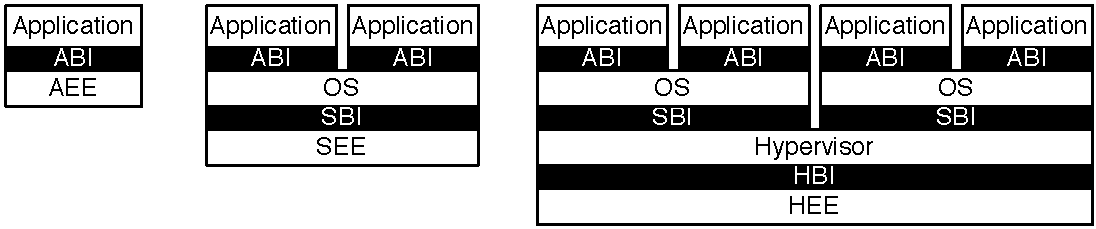
\includegraphics[width=\textwidth]{figs/privimps.pdf}
\caption{Different implementation stacks supporting various forms of
  privileged execution.}
\label{fig:privimps}
\end{figure}

\begin{commentary}
Our graphical convention represents abstract interfaces using black
boxes with white text, to separate them from concrete instances of
components implementing the interfaces.
\end{commentary}

The middle configuration shows a conventional operating system (OS)
that can support multiprogrammed execution of multiple
applications. Each application communicates over an ABI with the OS,
which provides the AEE.  Just as applications interface with an AEE
via an ABI, RISC-V operating systems interface with a supervisor
execution environment (SEE) via a supervisor binary interface (SBI).
An SBI comprises the user-level and supervisor-level ISA together with
a set of SBI function calls.  Using a single SBI across all SEE
implementations allows a single OS binary image to run on any SEE.
The SEE can be a simple boot loader and BIOS-style IO system in a
low-end hardware platform, or a hypervisor-provided virtual machine in
a high-end server, or a thin translation layer over a host operating
system in an architecture simulation environment.

\begin{commentary}
Most supervisor-level ISA definitions do not separate the SBI from the
execution environment and/or the hardware platform, complicating
virtualization and bring-up of new hardware platforms.
\end{commentary}

The rightmost configuration shows a virtual machine monitor
configuration where multiple multiprogrammed OSs are supported by a
single hypervisor.  Each OS communicates via an SBI with the
hypervisor, which provides the SEE.  The hypervisor communicates with
the hypervisor execution environment (HEE) using a hypervisor binary
interface (HBI), to isolate the hypervisor from details of the
hardware platform.

\begin{commentary}
The various ABI, SBI, and HBIs are still a work-in-progress, but we
anticipate the SBI and HBI to support devices via virtualized device
interfaces similar to virtio~\cite{virtio}, and to support device
discovery.  In this manner, only one set of device drivers need be
written that can support any OS or hypervisor, and which can also be
shared with the boot environment.
\end{commentary}

Hardware implementations of the RISC-V ISA will generally require
additional features beyond the privileged ISA to support the various
execution environments (AEE, SEE, or HEE).

\section{Privilege Levels}

At any time, a RISC-V hardware thread ({\em hart}) is running at some
privilege level encoded as a mode in one or more CSRs (control and
status registers).  Three RISC-V privilege levels are currently defined
as shown in Table~\ref{privlevels}.

\begin{table*}[h!]
\begin{center}
\begin{tabular}{|c|c|c|c|}
  \hline
   Level & Encoding & Name      & Abbreviation \\ \hline  
   0     & \tt 00   & User/Application & U     \\ 
   1     & \tt 01   & Supervisor & S           \\ 
   2     & \tt 10   & {\em Reserved} &            \\ 
   3     & \tt 11   & Machine    & M           \\ 
  \hline
 \end{tabular}
\end{center}
\caption{RISC-V privilege levels.}
\label{privlevels}
\end{table*}

Privilege levels are used to provide protection between different
components of the software stack, and attempts to perform operations
not permitted by the current privilege mode will cause an exception to
be raised.  These exceptions will normally cause traps into an
underlying execution environment.

The machine level has the highest privileges and is the only mandatory
privilege level for a RISC-V hardware platform.  Code run in
machine-mode (M-mode) is usually inherently trusted, as it has
low-level access to the machine implementation.  M-mode can be used to
manage secure execution environments on RISC-V.  User-mode (U-mode)
and supervisor-mode (S-mode) are intended for conventional application
and operating system usage respectively.

\begin{commentary}
The previous Hypervisor mode (H-mode) designed to support Type-1
hypervisors has been removed and the encoding space reserved as we are
focusing on hypervisor support via an extended S mode suitable for
both Type-1 and Type-2 hypervisors as described in
Chapter~\ref{hypervisor}.  The encoding space for H is reserved for
future use and to avoid backwards incompatible changes in bit
positions in various status regusters.  The bit positions might be
reused in the future for different Type-1 hypervisor support or
possibly additional secure execution modes.
\end{commentary}

Each privilege level has a core set of privileged ISA extensions with
optional extensions and variants.  For example, machine-mode supports
several optional standard variants for address translation and memory
protection.  Also, supervisor-mode can be extended to support Type-2
hypervisor execution as described in Chapter~\ref{hypervisor}.

Implementations might provide anywhere from 1 to 3 privilege modes
trading off reduced isolation for lower implementation cost, as shown
in Table~\ref{privcombs}.

\begin{commentary}
In the description, we try to separate the {\em privilege level} for
which code is written, from the {\em privilege mode} in which it runs,
although the two are often tied.  For example, a supervisor-level
operating system can run in supervisor-mode on a system with three
privilege modes, but can also run in user-mode under a classic virtual
machine monitor on systems with two or more privilege modes.  In both
cases, the same supervisor-level operating system binary code can be
used, coded to a supervisor-level SBI and hence expecting to be able
to use supervisor-level privileged instructions and CSRs.  When
running a guest OS in user mode, all supervisor-level actions will be
trapped and emulated by the SEE running in the higher-privilege level.
\end{commentary}

\begin{table*}[h!]
\begin{center}
\begin{tabular}{|c|l|l|}
  \hline
   Number of levels &  Supported Modes & Intended Usage \\ \hline  
   1     & M          & Simple embedded systems \\ 
   2     & M, U       & Secure embedded systems \\ 
   3     & M, S, U    & Systems running Unix-like operating systems\\ 
  \hline
 \end{tabular}
\end{center}
\caption{Supported combinations of privilege modes.}
\label{privcombs}
\end{table*}

All hardware implementations must provide M-mode, as this is the only
mode that has unfettered access to the whole machine.  The simplest
RISC-V implementations may provide only M-mode, though this will
provide no protection against incorrect or malicious application code.

\begin{commentary}
  The lock feature of the optional PMP facility can provide some
  limited protection even with only M-mode implemented.
\end{commentary}

Many RISC-V implementations will also support at least user mode
(U-mode) to protect the rest of the system from application code.
Supervisor mode (S-mode) can be added to provide isolation between a
supervisor-level operating system and the SEE.

A hart normally runs application code in U-mode until some trap (e.g.,
a supervisor call or a timer interrupt) forces a switch to a trap
handler, which usually runs in a more privileged mode. The hart will
then execute the trap handler, which will eventually resume execution
at or after the original trapped instruction in U-mode.  Traps that
increase privilege level are termed {\em vertical} traps, while traps
that remain at the same privilege level are termed {\em horizontal}
traps.  The RISC-V privileged architecture provides flexible routing
of traps to different privilege layers.

\begin{commentary}
Horizontal traps can be implemented as vertical traps that
return control to a horizontal trap handler in the less-privileged mode.
\end{commentary}

\section{Debug Mode}

Implementations may also include a debug mode to support off-chip
debugging and/or manufacturing test.  Debug mode (D-mode) can be
considered an additional privilege mode, with even more access than
M-mode. The separate debug specification proposal describes operation
of a RISC-V hart in debug mode.  Debug mode reserves a few CSR
addresses that are only accessible in D-mode, and may also reserve
some portions of the physical memory space on a platform.
